%********************************************************************
% Kapitel 3
%*******************************************************
\chapter{Architecture}
\label{ch:Architecture}

\section{Overview}

In general, the application consists of two separate applications. For once, we have the React frontend which is running in a browser. On the other side there is the Spring Boot backend application server. Usually the user will use the \ac{UI} to display data which the frontend fetches from the backend. Backend also does handle authentication as previously mentioned. \ac{IETF} draft \textit{OAuth 2.0 for Browser-Based Apps} describes how such architectures look like and even mentions React and Spring Boot as an example in section 6.2. \textit{JavaScript Applications with a Backend}.

\begin{figure}[bth]
    \centering
    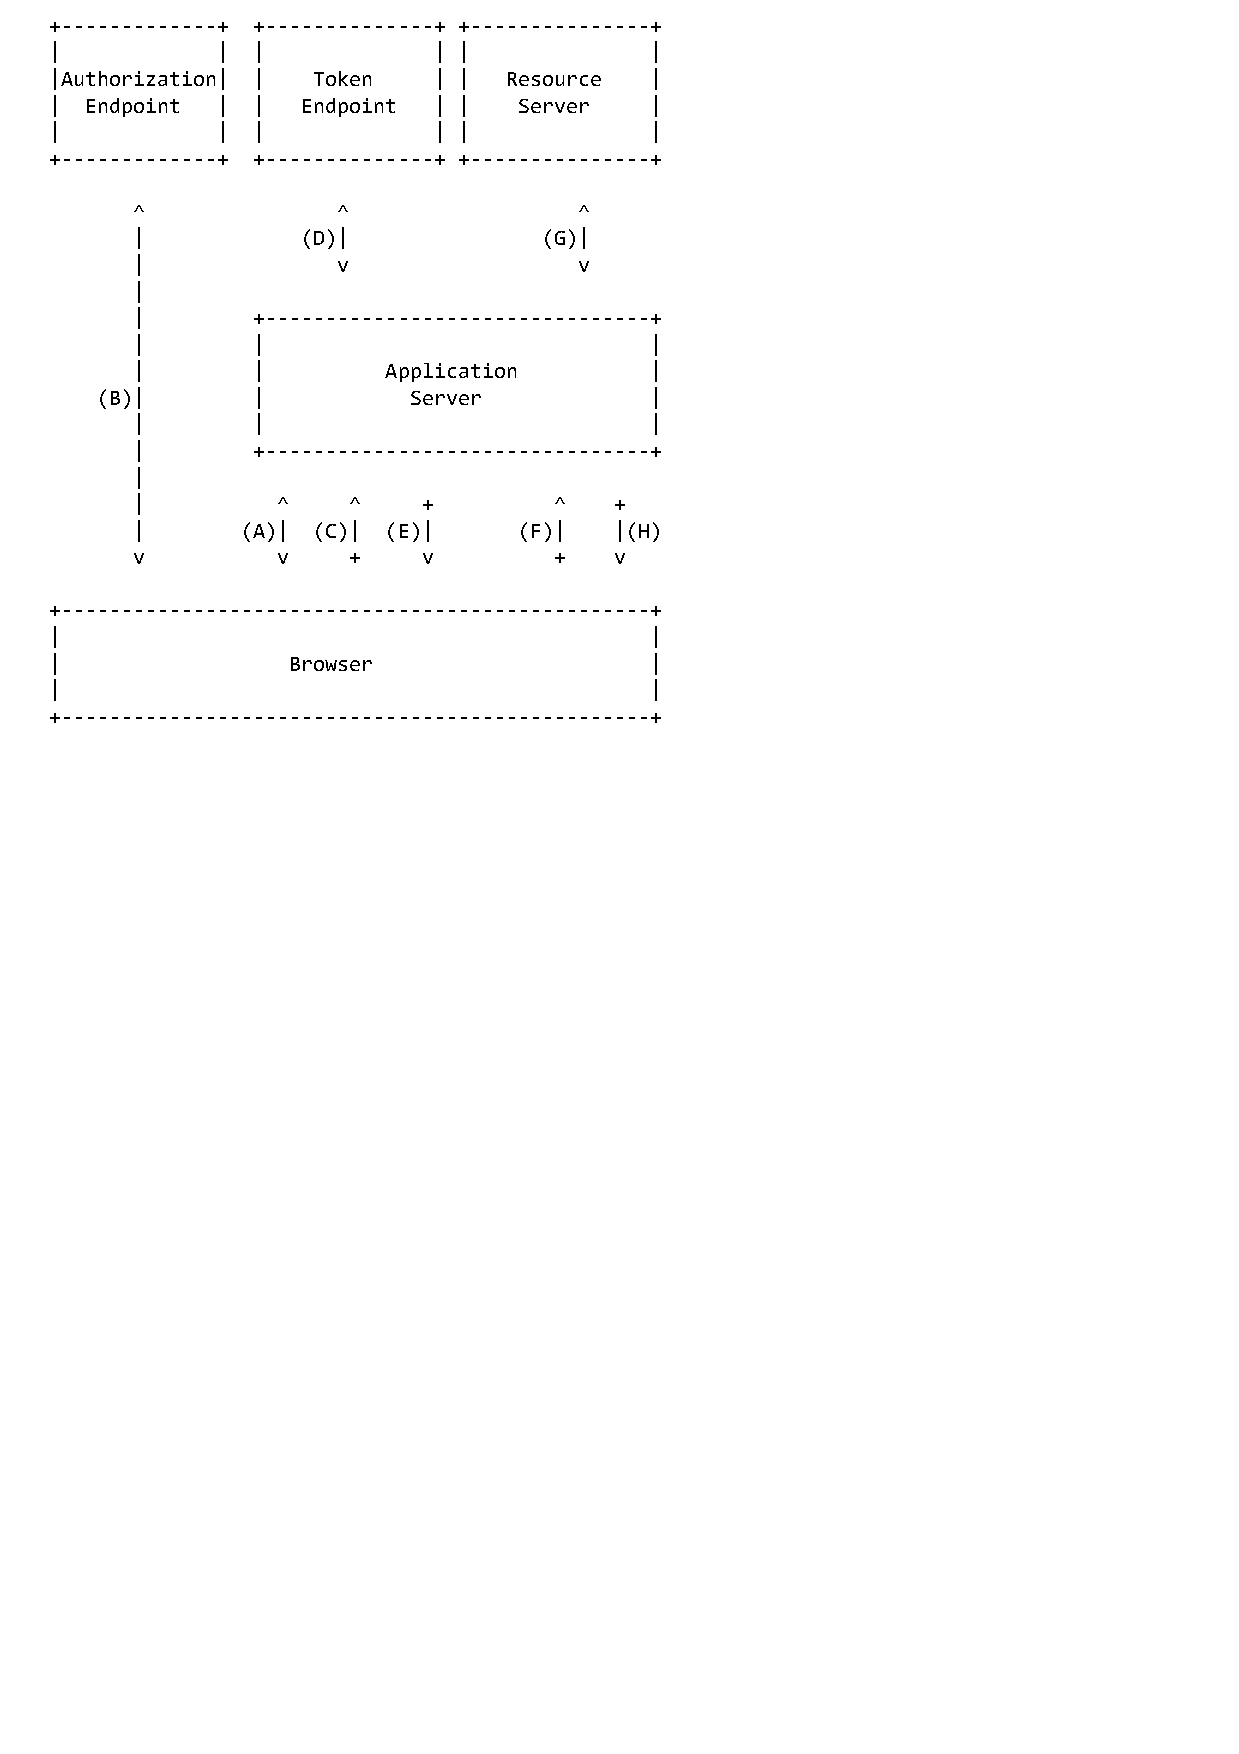
\includegraphics[width=0.7\textwidth]{Graphics/Chapter3/ietf-oauth-draft.pdf}
    \caption{Architecture from an authentication point of view \cite[Section~6.2]{IetfOauthDraft}}
\end{figure}

In our case, the application server is Spring Boot and the authorization endpoint is the Spotify login page (see \autoref{fig:SpotifyLogin}). The token endpoint is a Spotify API endpoint and is configured in the Spring Boot application. The only difference to above figure is that the backend application is not setup to serve frontend files (the resource server part). This is because we usually would run the React and Spring Boot application separately during development. Do note that not serving frontend files from the backend application comes with some drawbacks though. For example, we had to disable \ac{CSRF} protection as it does only work if the backend serves frontend files. This brings us to the actual high-level architecture overview from a user perspective.

\begin{figure}[bth]
    \centering
    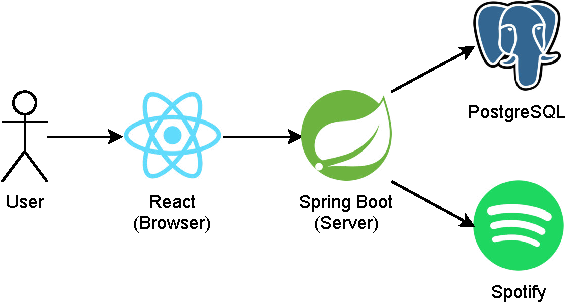
\includegraphics[width=0.8\textwidth]{Graphics/Chapter3/architecture-overview.pdf}
    \caption{Architecture from a user point of view}
\end{figure}

As one can see, the backend application handles communication to the database (PostgreSQL) as well as Spotify (for fetching data and authentication). Frontend and backend exchange data using \ac{HTTP}.

\section{Backend}

The backend application is powered by the Spring Framework and basically serves as an intermediate between what the user sees in the frontend and the data in our database as well as the data that the Spotify API provides. In fact, the backend application even provides an endpoint which just relays requests to the Spotify API so you theoretically could talk to the whole Spotify Web API through one \ac{HTTP} endpoint.

But of course the application does more than that. First, a user will have to authenticate. We did setup Spring Security and its OAuth2 client to handle authentication. Spring Security will also handle redirection after successful authentication, \ac{CORS} and access to the Spotify API as it requires a valid OAuth Token.

Furthermore, backend will handle querying the database using Spring Data and transforming that data into a \acs{JSON} response enriched with data fetched from the Spotify Web API. Most of the codebase will account for such functionality so let us go into more detail. For starters, the application follows a layered architecture approach and classes are packaged by feature. Those design decisions are inspired by \ac{DDD} and you will quickly notice that our packages represent different domains of the application that you can observe in the \ac{UI}, namely:

\begin{description}
    \item[discover] This package handles requests that want to fetch new recommendations. It will call the PostgreSQL functions and will also query the Spotify Web API for track, album and artist details.
    \item[rating] This package handles rating requests in case you change the star rating of a track, album or artist in frontend.
    \item[recent] This package handles requests that want to fetch recently-played tracks. They will display for the user to see in the frontend.
\end{description}

Besides those three main packages there are also some other important packages:

\begin{description}
    \item[dataset] This package does not provide any endpoints but is used to convert parts of the dataset from \acs{JSON} to \acs{CSV} so it can be imported into PostgreSQL.
    \item[spotify] This package contains the aforementioned endpoint that will delegate any requests including their headers and body to the Spotify Web API. It most importantly also includes a class that serves as a client to the API so that other packages can simply reuse it (\texttt{SpotifyApi}).
    \item[user] This package provides an endpoint for frontend so it can check if a user is logged-in.
\end{description}

The other two remaining packages \textbf{configuration} and \textbf{utils} do contain obligatory Spring application configuration and utility classes that can be used by all other domains. Most noteworthy, it does contain a routing configuration that is responsible for routing \ac{HTTP} requests. It also does contain classes that handle caching. Caching is done for outbound \ac{HTTP} requests to the Spotify API using a high-performance in-memory cache called \href{https://github.com/ben-manes/caffeine}{Caffeine}. The cache is configured to clear entries five minutes after write so that recently-played tracks are still somehow up to date.

\begin{figure}[bth]
    \centering
    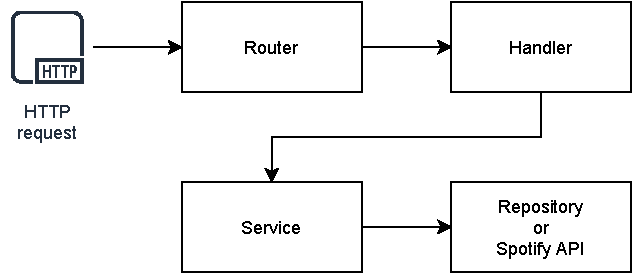
\includegraphics[width=0.8\textwidth]{Graphics/Chapter3/backend-layers.pdf}
    \caption{Different layers in the backend application}
\end{figure}

In terms of layers we pretty much do follow the \ac{DDD} approach of a distinct application, domain and infrastructure layer. An inbound request will get handled by the application layer consisting of a router and handler. You might know this combination of router and handler as a \texttt{RestController} in the traditional servlet stack of Spring. Anyway, the router contains the path mappings and the handler will delegate tasks to the appropriate service layer. The service layer then will do the actual work and do transformation of data it fetches from the infrastructure layer. That final layer consists of a Spring Data repository or an other database access mechanism (e.g. templates) but it could also be our \texttt{SpotifyApi} implementation that provides access to Spotify Web API endpoints.

\section{Frontend}

Frontend builds upon the popular React JavaScript library. It was deliberately chosen in favor of Angular and Vue.js as we do like its approach of building user interfaces the most. React uses a component-based approach where \acs{HTML} pages consist of reusable components which each manage their own individual state. Common examples for a component on a webpage are the header or footer section of the page which in itself each can contain more sub-components.

\begin{figure}[bth]
    \centering
    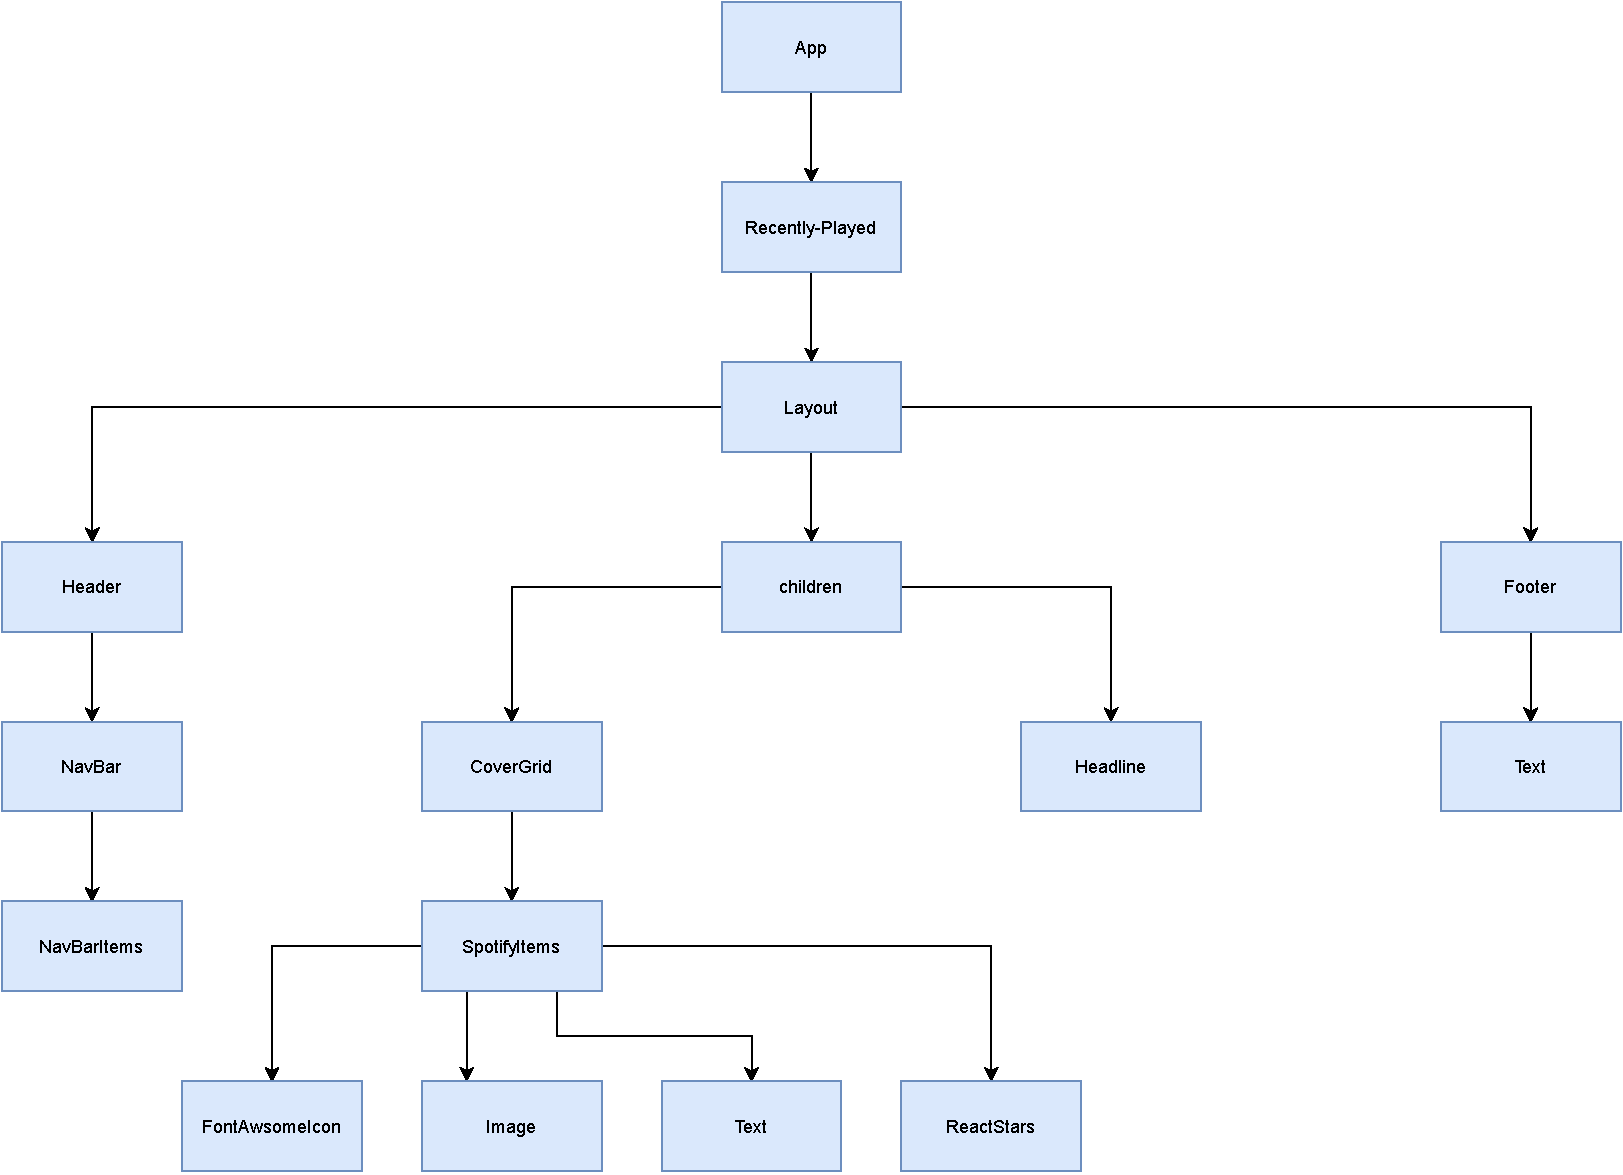
\includegraphics[width=1.0\textwidth]{Graphics/Chapter3/frontend-component-tree.pdf}
    \caption{Exemplary component tree of the recently played page}
\end{figure}

Components do store some of the state using a library called Redux. Redux is configured to store data in local storage of your browser which means you can look at it using the browser developer tools (under Application > Storage > Local Storage). The data that we store in Redux is fetched from the backend application asynchronously using Redux Thunk and axios. The latter is responsible for doing \ac{HTTP} requests using a session cookie the user will receive from the backend application after logging in successfully.

Other than the backend application, the frontend application is not packaged by feature but packaged by layer:

\begin{description}
    \item[api] Does contain a single file that handles access to the backend using axios.
    \item[app] Does contain application configuration for React Router as well as Redux.
    \item[components] Does contain components that the user actually will see on the webpage.
    \item[reducers] Does contain reducer definitions for Redux. They describe how the state looks like and provides functions to update the state.
    \item[routes] Does contain React Router routes that primarily assemble a full page using components from the previously mentioned components directory.
\end{description}

The \acs{CSS} framework of choice is Bulma. Additional libraries that provide \acs{CSS} files are the Font Awesome icon library as well as the Swiper slider library. Also, components can define component-specific \acs{CSS} in a \texttt{.module.css} file like \texttt{Avatar.module.css} does for the user avatar component. Additionally, we had to override some Bulma styles as the React library that does provide Bulma components is unfortunately slightly outdated.
